\documentclass[11pt,a4paper]{article}

\setlength {\marginparwidth }{2cm}

\usepackage[margin=2.5cm]{geometry}
\usepackage{todonotes}
\usepackage[automake]{glossaries}
\usepackage{graphicx}
\usepackage{microtype}
\usepackage{listings}
\usepackage{color}
\usepackage{amssymb,amsmath}
\usepackage{mathpazo}
\usepackage{accents}
\usepackage{longtable,booktabs}
\usepackage{dcolumn}
\usepackage{pgf}
\usetikzlibrary{shapes.geometric}
\usetikzlibrary{matrix}
\usepackage{natbib}
\usepackage{hyperref}
\usepackage[capitalise,noabbrev,nameinlink]{cleveref}
\hypersetup{
  pdftitle={Input-Endorsers Solution Primer},
  pdfborder={0 0 0},
  breaklinks=true
}
\graphicspath{ {./images/} }

\definecolor{dkgreen}{rgb}{0,0.6,0}
\definecolor{gray}{rgb}{0.5,0.5,0.5}
\definecolor{pink}{rgb}{0.92,0.2,0.86}

\lstset{frame=tb,
  language=Haskell,
  aboveskip=3mm,
  belowskip=3mm,
  showstringspaces=false,
  columns=flexible,
  basicstyle={\ttfamily},
  numbers=none,
  numberstyle=\tiny\color{pink},
  keywordstyle=\color{pink},
  commentstyle=\color{pink},
  stringstyle=\color{pink},
  breaklines=true,
  breakatwhitespace=true,
  tabsize=3
}

\DeclareMathOperator{\dom}{dom}
\newcommand\restrict[2]{\left.#1\right||_{#2}}
\newcommand\deltavar[1]{\accentset{\Delta}{#1}}

\makeglossaries
\newglossaryentry{rb}
{
    name={Ranking Block},
    description={a block which is responsible for transporting references to \glsplural{ib}}
}
\newglossaryentry{ib}
{
    name={Input Block},
    description={a block which is responsible for transporting transactions (or transaction references)}
}
\newglossaryentry{tier}
{
    name={Tier},
    description={a grouping which attempts to classify priority of transport of \glsplural{ib}}
}
\newglossaryentry{tx}
{
    name={Transaction},
    description={an object representing UTxOs being spent (with or without a script context), and a destination address} 
}

\begin{document}

\title {Input-Endorsers Solution Primer \\
       {\large \sc An IOHK discussion paper}}
\date  {Version 0.1, 16th May 2022}
\author{John Woods         \\ {\small \texttt{john.woods@iohk.io}} \\
                              {\small \texttt{john@postquantum.dev}} \\
}

\maketitle

\section{Purpose}
The purpose of this document is to provide a macroscopic view of the current state of 
research, a potential architectural design, and highlight possible design pitfalls 
with regard to the upcoming \emph{Input-Endorsers} protocol enhancement. \\ 

The goal of the Input-Endorsers is to minimize under-utilization of Cardano's system resources.
As of writing, approximately 25\% ($5$ seconds out of each $20$ second period) are currently being used to process
transactions. The remaining 75\% of the time is spent idle, filling mempool, or dedicated to other tasks
which do not contribute to the bandwidth of the network.

Thus, the goal with the introduction of Input-Endorsers is to achieve a higher transaction throughput
by utilizing resources more efficiently, and more effectively. This change (which will touch the three 
major system components: Consensus, Ledger \& Network) will also pave the way for the introduction of tiered
pricing, which is also discussed herein. \\

This document will look at hypothetical requirements (motivation), highlight the a potential high-level
architecture, and finally, shine a light on some potential "footguns" which the implementation should consider. \\

The target audience for this document is Engineering, and it should be considered a disambiguation paper 
rather than a design document. As of writing, Research on Input Endorsers is still ongoing, thus, design 
decisions are still in flux.
\pagebreak

\tableofcontents

\pagebreak

\section{Acknowledgements}
The ideas presented herein are inspired by and based on discussions with
people from the research and engineering groups, specifically: Aggelos Kiayias, 
Giorgos Panagiotakos, Matthias Fitzi, Sandro Coretti, Philip Lazos, Duncan Coutts,
Neil Davies, Benjamin Beckmann \& Vitor Silva.

\pagebreak

\section{Context}
Input Endorsers are a major enhancement to the Cardano consensus protocol, Ouroboros.
Input Endorsers decouple consensus \& transaction diffusion. Input Endorsers represent 
Cardano's next-generation layer 1 scaling technology. \\ \\
It's recognized that Cardano's resources are currently under-utilized:

\begin{itemize}
  \item Less than 25\% of time is spent creating and transmitting blocks/transactions.
  \item More than 75\% of time is spent idle, waiting for a new block, or filling mempool.
\end{itemize}

\begin{figure}[ht]
  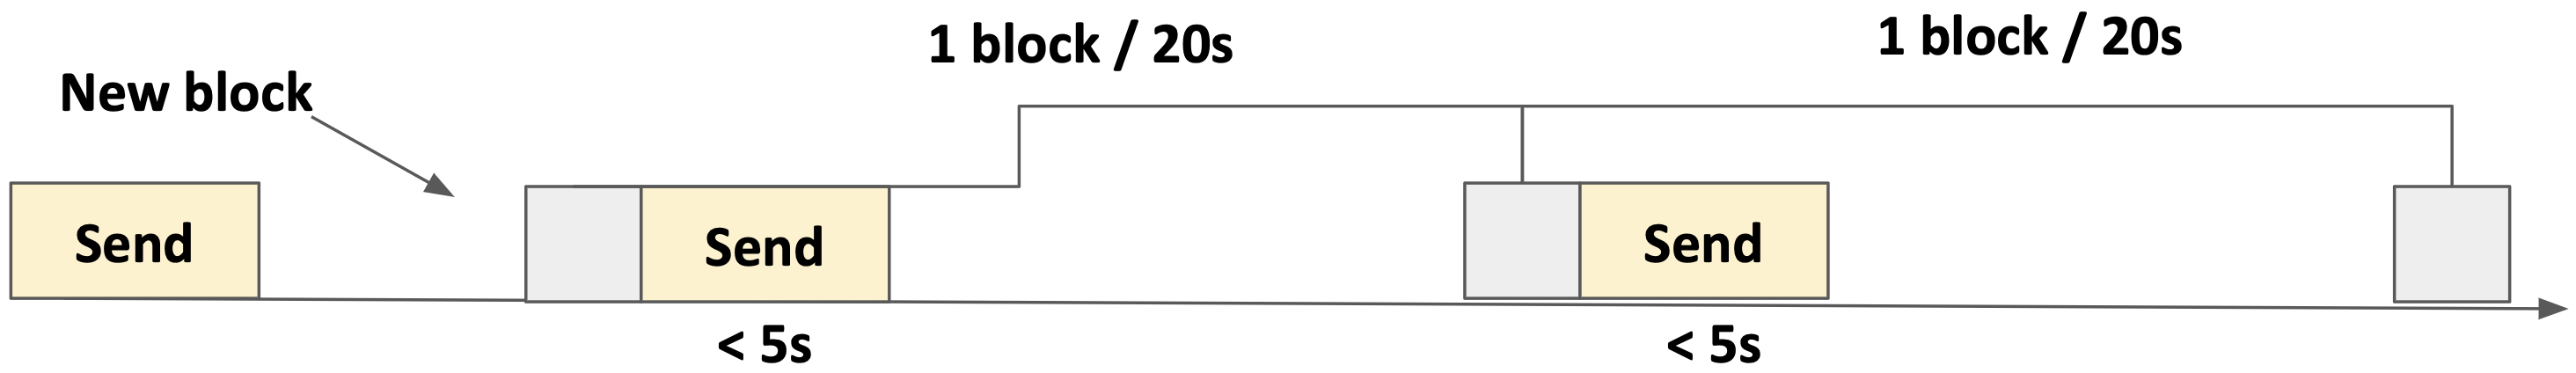
\includegraphics[width=\linewidth]{current_usage.png}
  \caption{current resource utilization}
  \label{fig:current utilization}
\end{figure}

We need to achieve higher throughput by utilizing resources more effectively.
The key insight with Input Endorsers is the realization that with a single block
type, said block is responsible for both transaction propagation (as transactions are a 
given block's payload) \emph{and} for consensus. However, if we introduce a scheme which 
\emph{decouples} consensus from transaction propagation, achieved by employing \emph{two} 
different block types, we can then reduce low resource utilization, and achieve higher
transaction throughput. \\

As we cannot simply increase block production to increase throughput (due to the danger of increased 
forks/height battles), thus consider the following scheme, which depicts a construction which may 
be used to achieve a more effective utilization of the network's resources:

\begin{figure}[ht]
  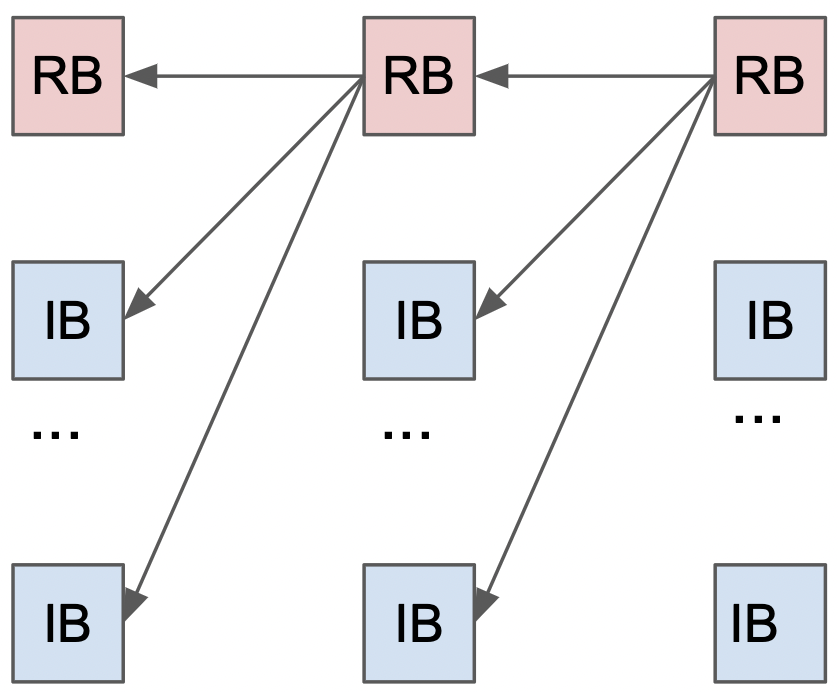
\includegraphics[width=0.4\textwidth]{ie_structure.png}
  \centering
  \caption{proposed block re-structure}
  \label{fig:proposed re-structure}
\end{figure}

\pagebreak

\textbf{Input Endorsers} introduces \emph{two} categories of blocks:

\begin{itemize}
  \item \emph{\glsplural{rb}}: responsible for consensus. 
    \subitem \textbf{Payload}: \gls{ib} references.
  \item \emph{\glsplural{ib}}: responsible for transaction propagation.
    \subitem \textbf{Payload}: \gls{tx} references.
\end{itemize}

\textbf{\glsplural{rb}} will use reference semantics to reference \glsplural{ib}, \glsplural{rb} will still employ
the "longest chain" rule. They will be solely responsible for consensus and shall have a "low"
production rate, which is expected to be similar to our current block production rate, approximately 
one block every $20$ seconds. \glsplural{rb} will have low resource utilization. \\

\textbf{\glsplural{ib}} \emph{should} also use reference semantics, which is discussed further herein (\emph{note: in 
preliminary research artefacts \glsplural{ib} employed value semantics rather than reference semantics}) \glsplural{ib} 
will carry a payload of transaction references, and will be solely responsible for propagation of transactions. The 
actual transaction data will be propagated separately. This approach is being considered to:

\begin{itemize}
  \item Reduce transmission of duplicate data over the network graph.
  \item Reduce the intersection size (overlap) of \glsplural{ib}.
\end{itemize}

Both of these topics are discussed further herein. \glsplural{ib} will have a "high" production rate, which is expected to
yield a significant increase in throughput. \\


\glsplural{rb} will order (serialize) \glsplural{ib}.
\glsplural{ib} will order transactions.

The scheme described above may be visualized in a timeline as:

\begin{figure}[ht]
  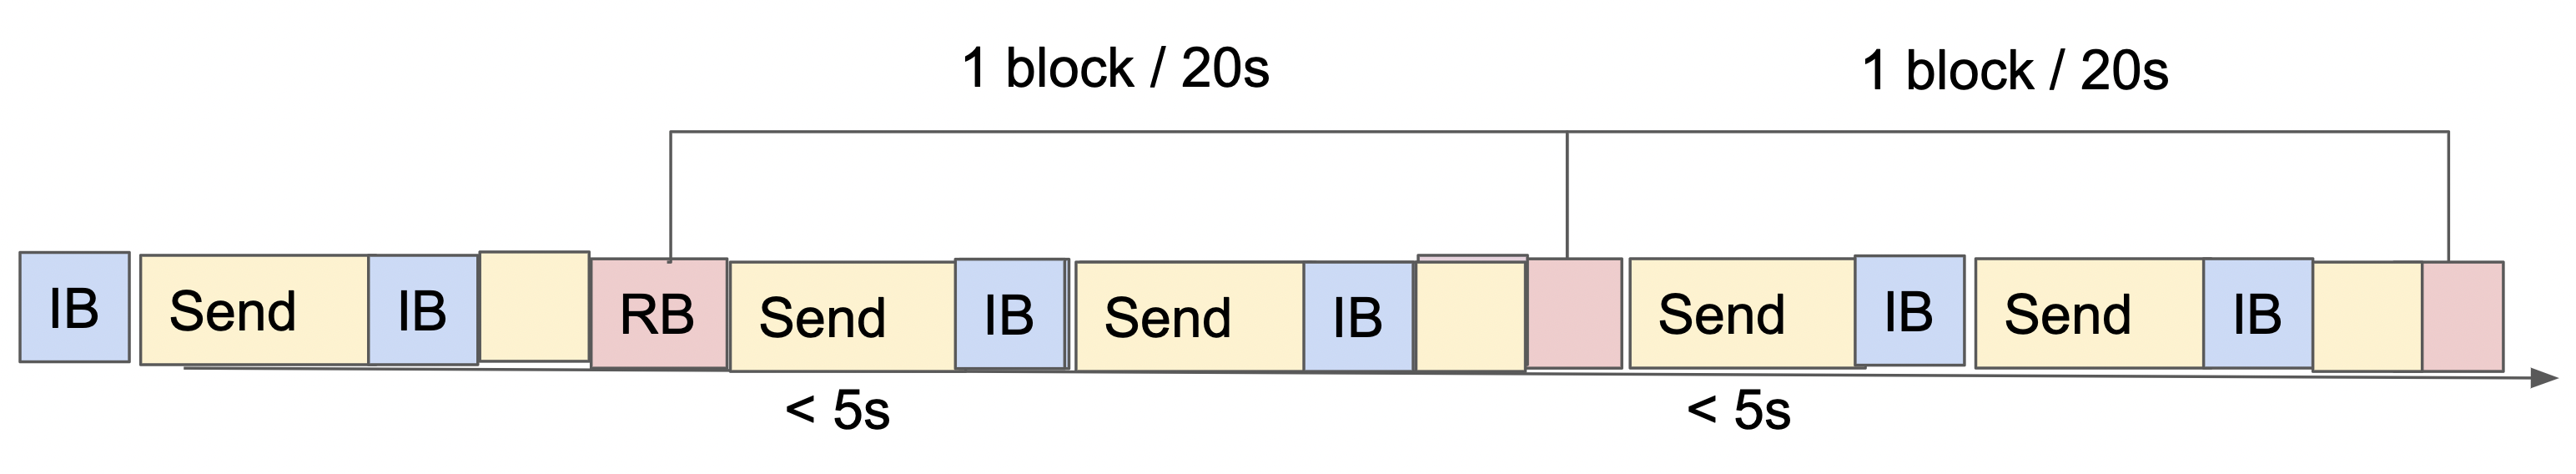
\includegraphics[width=\linewidth]{proposed_usage.png}
  \caption{proposed resource utilization}
  \label{fig:proposed utilization}
\end{figure}

\pagebreak

\section{Solution discussion}
Following is a high-level view into aspects of the technical architecture required for Input Endorsers.
In this section we explore and discuss technical cornerstones of the design, some of which are a radical
departure from our current implementation of Ouroboros, and indeed the Ledger rules. \\ 

Additionally, it is important to note that the following should be considered a hypothetical approach, 
not a canonical design document. Ultimately our goal is to deliver on the functional and non-functional 
requirements, without adding unnecessary complexity to the system components. \\

Input Endorsers provides high throughput by design. Thus, the engineering challenge changes from \emph{"How do we
increase the throughput of the system?"} to \emph{"How do we maximize efficacy and eliminate redundant data propagation?"} \\

In following sections we will discuss technical approaches which may be used to solve this challenge.

\subsection{VRF Usage}
Both \glsplural{ib} \& \glsplural{rb} will be produced using the same VRF (verifiable random function) mechanism 
as the current implementation of Ouroboros. That is, block producers will be \emph{selected} using a VRF. 



\subsection{"Colouring"}

\subsection{Mempool Design}
Mempool will see significant changes, though importantly it will maintain a \emph{FIFO} structure.

\subsection{Blockchain Structure}

\subsection{Attacks/Fragility}

\subsection{Tiered Fees}



\pagebreak


\section{Conclusion}

\subsection{Benefits:}
\subsection{Limitations:}


\pagebreak
\printglossaries
\end{document}